 % this file is prim_pollard.tex
	 % this file is prim_tools.tex
 
  
  \section{Pollard Rho Methode}
  \label{sec:pollard}
  \subsection{Geburtstagsproblem}
  Die Idee des Geburtstagsproblems ist die Frage, wie hoch die Wahrscheinlichkeit auf einem Geburtstag mit $N$ Personen ist, dass zwei am gleichen Tag Geburtstag haben.\\
  Eine M\"oglichkeit das Problem einfacher zu machen ist, stattdessen das inverse Problem zu betrachten, also wie hoch die Wahrscheinlichkeit $(P)$ ist, dass kein Geburtstag doppelt vorkommt.\\
  Bei einem Besucher ist die Wahrscheinlichkeit
  \[P(1)=\frac{356}{356}\] 
  da alle $356$ Tage zur Wahl stehen. Bei zwei Besuchern ist die Wahrscheinlichkeit 
  \[P(2)=\frac{356}{356}\cdot \frac{364}{365}\]
  bei drei Besuchern gilt  
  \[P(3)=\frac{356}{356}\cdot \frac{364}{365} \cdot \frac{363}{365}\]
  Im Allgemeinen gilt: 
  \[P(N)= \frac{365 \cdot 364 ... (365-N+1)}{365^N}\]
  Da wir gro\ss e Primzahlen betrachten werden interessiert uns auch das Verhalten des Geburtstagsproblems f\"ur gro\ss e $N$.
  Beim Betrachten von vielen Geburtstagen mit $N$ Personen, liegt, f\"ur gro\ss e N, die Zahl der Wiederholungen die man durchschnittlich braucht um einen doppelten Geburtstag zu erhalten bei: 
  \[\sqrt{\frac{\pi \cdot N}{2}}\]
  
  \subsection{Hase Igel Algorithmus}
  Der Hase Igel Algorithmus wird benutzt, um Zyklen in Folgen zu finden. Die Idee ist, die Folge mit zwei Zeigern zu durchlaufen, dem Hase und dem Igel, die auf dem gleichen Feld starten. Falls es einen Zyklus in der Folge gibt, werden sich Hase und Igel irgendwann wieder treffen, da der schnellere Hase den langsameren Igel einholt und \"uberrundet.
  \subsubsection{Beispiel}
  In diesem Beispiel ist eine Folge zu sehen, die einen Zyklus beinhaltet. 
  
    \begin{figure}[!h] 
    	\centering
    	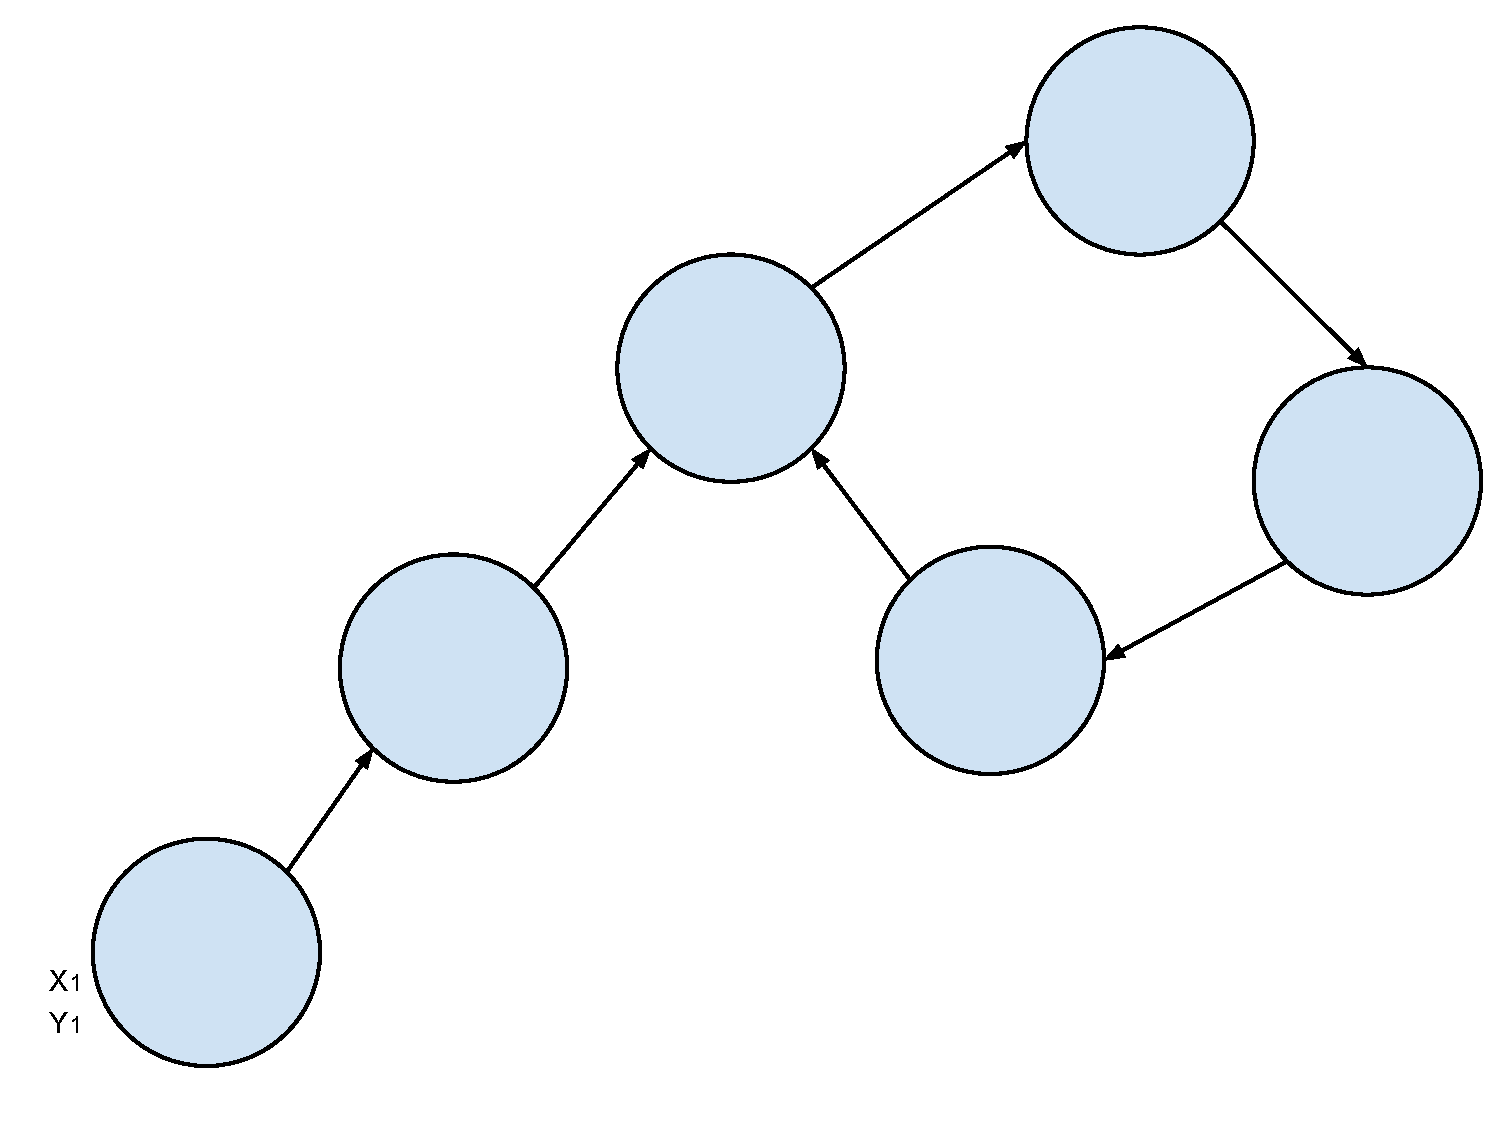
\includegraphics[width=0.7\linewidth]{Rho1}
    	\caption{Schritt 1}
    	\label{fig:Rho1)}
    \end{figure}
    
    Der Hase, hier dargestellt durch Y und der Igel, hier dargestellt durch X starten an der gleichen Position. Der Igel bewegt sich um ein Element, der Hase um zwei Elemente fort.

  \begin{figure}[!h] 
  	\centering
  	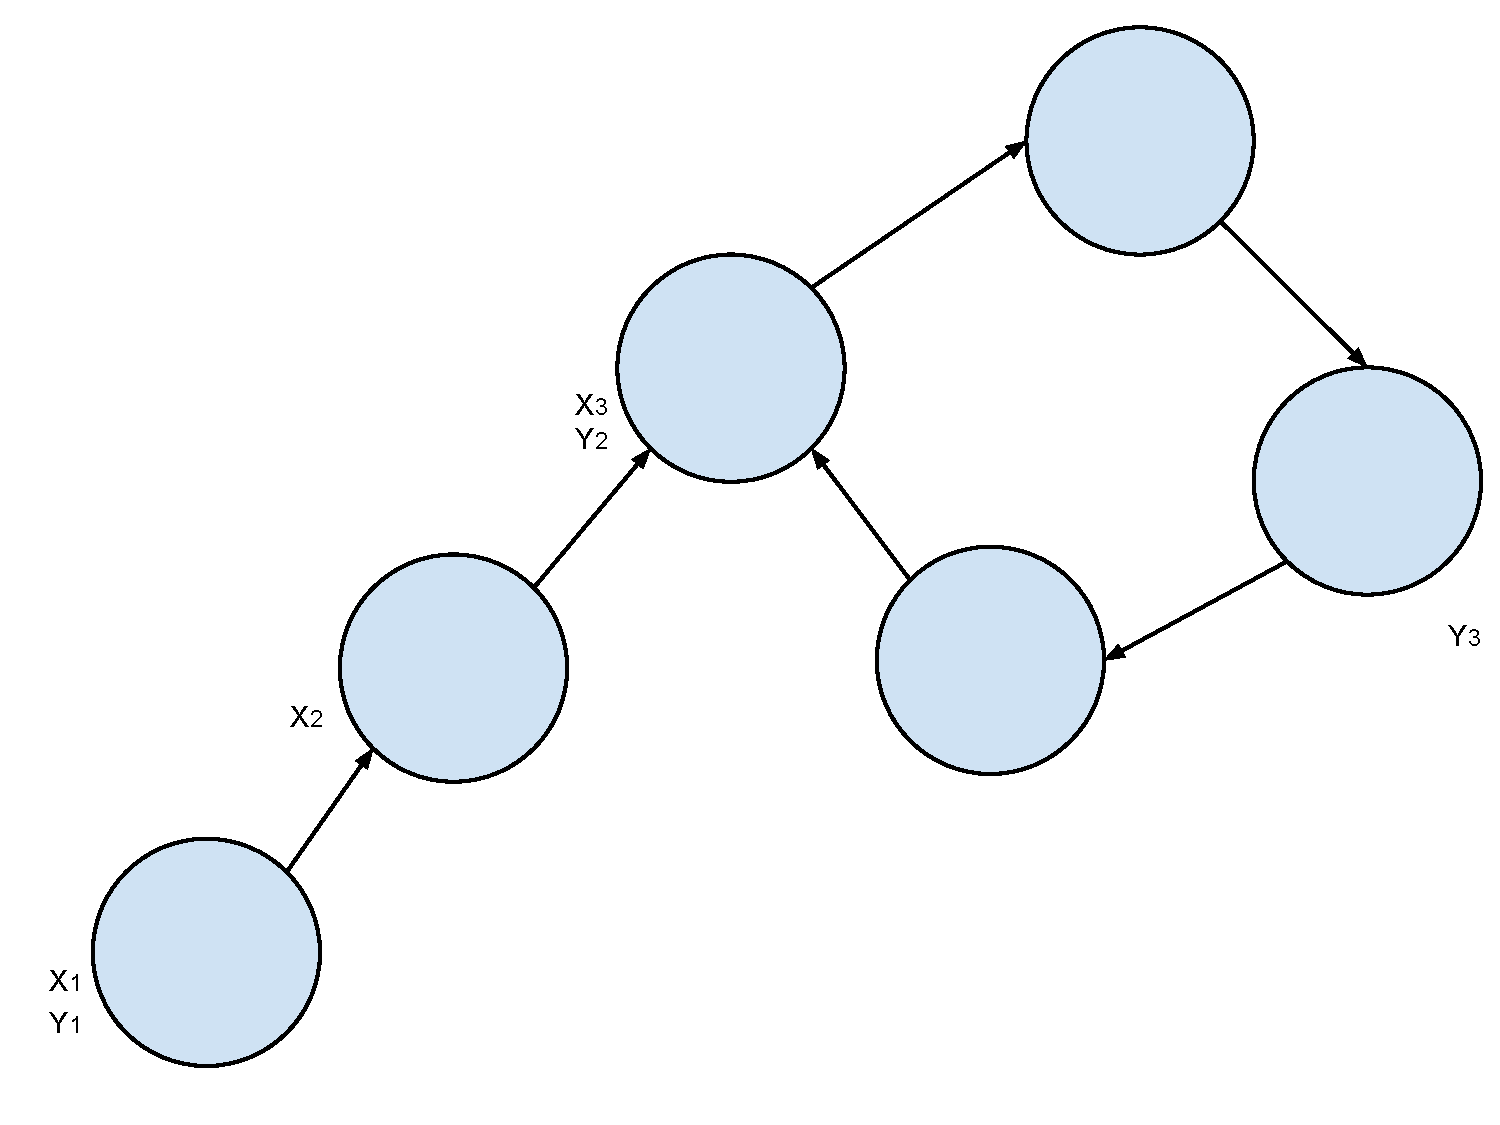
\includegraphics[width=0.7\linewidth]{Rho2}
  	\caption{Schritt 2}
  	\label{fig:Rho2)}
  \end{figure}
  
  Das ist der Zustand, bevor der Hase das erste mal im Kreis l\"auft. Es ist zu erkennen, dass der Hase doppelt so weit ist, wie der Igel.
  
    \begin{figure}[!h] 
    	\centering
    	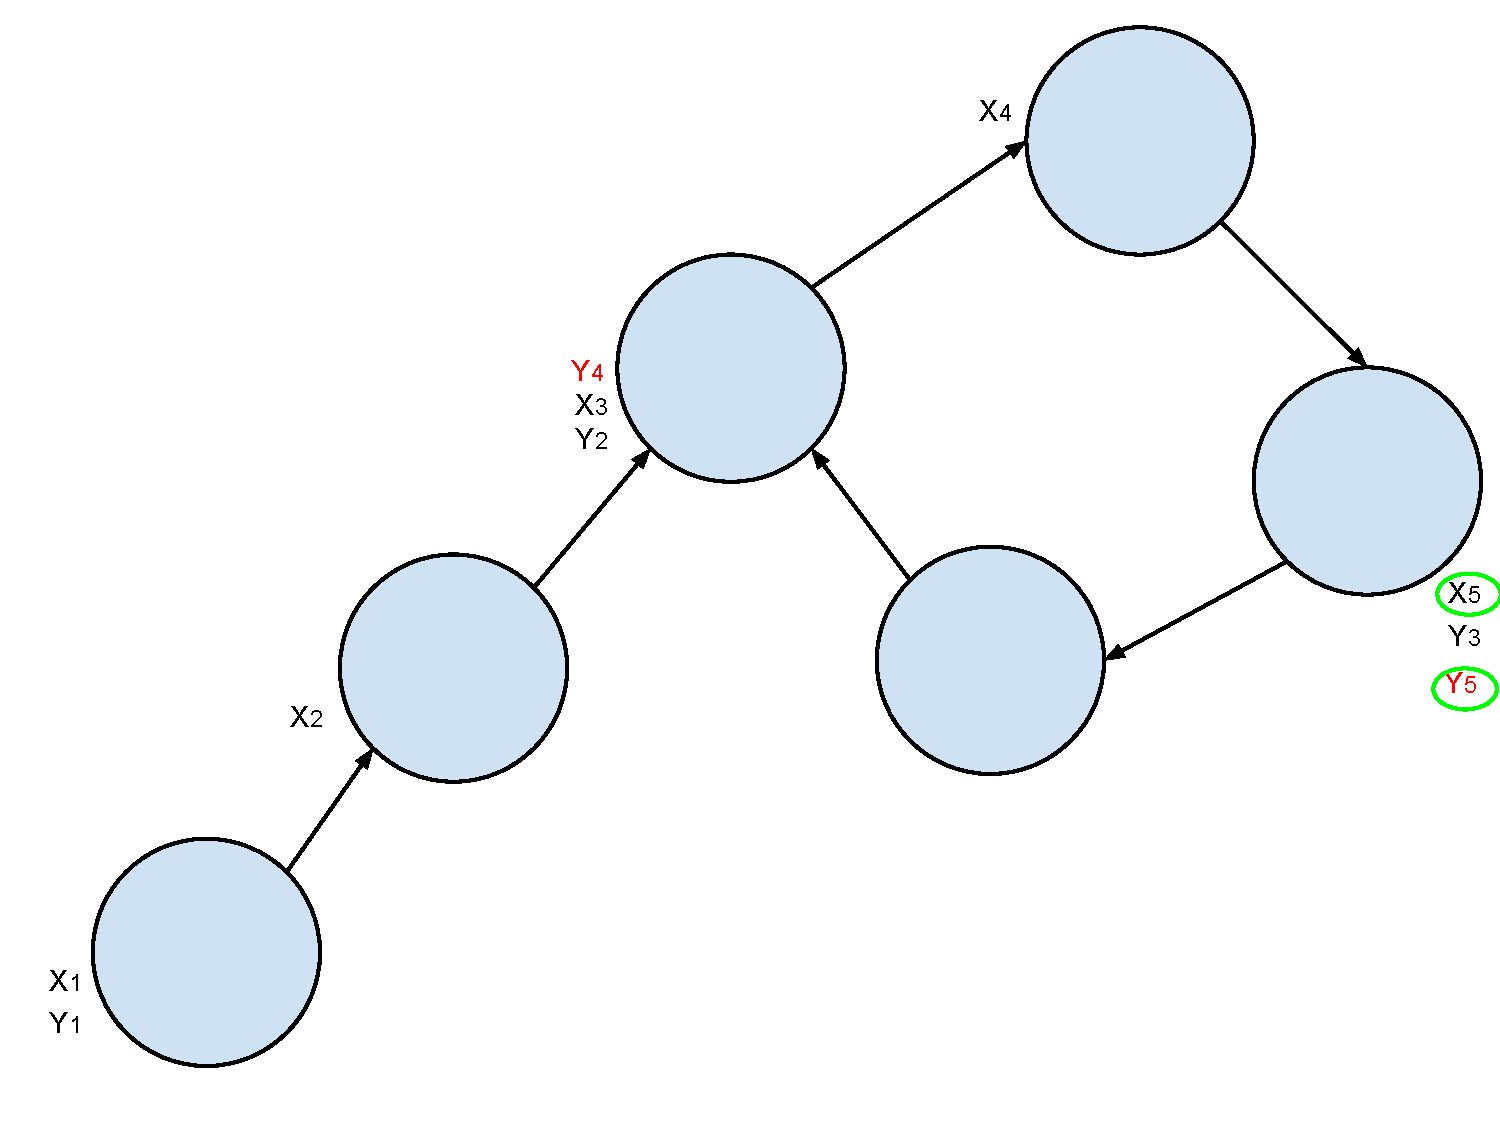
\includegraphics[width=0.7\linewidth]{Rho3}
    	\caption{Schritt 3}
    	\label{fig:Rho3)}
    \end{figure}
    Dies ist der Zustand, wenn Hase und Igel sich treffen. Die roten Zahlen zeigen, dass der Hase im Kreis l\"auft und die gr\"un eingekreisten Zahlen zeigen, dass Hase und Igel sich in ihrem f\"unften Schritt treffen. 

  \subsubsection{Mathematik}
  \begin{itemize}


  	\item Sei $M$ eine endliche Menge mit der Abbildung $f : M \rightarrow M$. Die Menge $M$ wird im Beispiel durch die Kreise dargestellt, die Abbildung $f$ durch die Pfeile, die die Kreise verbinden.
  	
  	\item Man w\"ahle $x_0 \in M$ und erzeuge die Folge $x_0, x_1, x_2,...$ mit $x_{i+1} = f(x_i)$. Dies wird im Beispiel durch den Igel dargestellt, der sich entlang der Pfeile mit einer Schrittweite von $1$ durch die Menge bewegt.
	
  	\item $\exists \ i,j \in \mathbb{N}$, sodass $i \not= j$ und $x_i = x_j$ gilt. Hiermit wird gesagt, dass es einen Zyklus gibt. Wenn der Igel zwei mal auf das gleiche Feld kommt, muss er im Kreis gegangen sein.
  	
  	\item Die Folge $y_0, y_1, y_2,...$ gegeben durch $y_0=x_0$ und $y_{i+1}=f(f(y_i))$ ist gleich der Folge $x_0,x_2,x_4,...$.\\
  Hiermit wird der Hase beschrieben, der sich doppelt so schnell bewegt wie der Igel. 
  	
  	\item Es gibt ein $c>0$, sodass $x_c=x_{2c}$.\\
  	Dies ist die Bedingung daf\"ur, dass es m\"oglich ist, dass sich Hase und Igel wieder treffen und zwar wenn beide gleich viele Schritte gemacht haben. $c$ f\"ur den Igel, $2c$ f\"ur den Hasen, da der Hase eine doppelt so gro\ss e Schrittweite hat wie der Igel.
  \end{itemize}
  
  Ein Beweis f\"ur diesen Algorithmus wird in Abschnitt \ref{sec:pollardBeweis} gef\"uhrt.
 	\subsection{Pollard Rho Algorithmus}
 	\subsubsection{Kongruenz modulo p}
 		Bevor wir mit dem n\"achsten Algorithmus anfangen k\"onnen, brauchen wir noch ein weiteres Werkzeug.\\
	 	Modulo Rechnen sollte bekannt sein. Weniger bekannt ist aber die Kongruenz $\pmod p$.
 	 
		\[a \equiv b \pmod p \Leftrightarrow p|(a-b)\]
		Gesprochen wird es: a ist kongruent b modulo p. wenn zwei Zahlen kongruent modulo p sind, bedeutet es, dass sie beim modulo nehmen mit p den gleichen Rest haben. Dies f\"uhrt wie oben beschrieben dazu, dass die Differenz von a und b durch p teilbar ist. Diese Eigenschaft wird durch folgende Umformung noch einmal 	verdeutlicht:
		\[a \equiv b \pmod p \Leftrightarrow a=p\cdot x +r,\ \ \ b= p\cdot y +r\]

		\[a-b=p(x-y)+(r-r)=p(x-y)\]

		\[p|p(x-y)\]

 	\subsubsection{Idee}
 	
 	  	Die Idee f\"ur den Algorithmus basiert auf folgender Schlussfolgerung: \\
 	  	Sei $n$ eine zusammengesetzte Zahl und $p$ ein Primfaktor von $n$.\\
 		Gesucht sind $a, b$, sodass:

  		$a \equiv b \pmod p \Leftrightarrow p|a-b$ \\
 		Daraus folgt $1<ggT(a-b,n) \leq  n$. \\Wenn $a\not = b$ gilt, ist $ggT(a-b,n)$ ein nichttrivialer Primfaktor von $n$.\\
 		\newline
		Der interessante Teil hierbei ist, die Folgerung, dass wenn $a \equiv b \pmod p$ gilt, auch $1<ggT(a-b,n) \leq  n$ gilt. Dies ist sehr einfach zu erkl\"aren, wenn man die Folgerung $a \equiv b \pmod p \Leftrightarrow p|a-b$ betrachtet. $p$ ist Teiler von n und von $a-b$. Da $p$ eine Primzahl ist, ist sie gr\"o\ss er als $1$ und maximal $n$ da sie $n$ teilt.
  
  	\subsubsection{Algorithmus}
  	Der Algorithmus funktioniert wie folgt:
 \begin{itemize}
 	\item Sei $f(x)$ eine ganzzahlige Polynomfunktion und $s \in \mathbb{Z}$.
 
 	\item Man erzeuge eine Folge von Pseudozufallszahlen mit: 
  	\[ 	x_0= s,  x_{i+1}=f(x_i) \pmod n  \]
	Die Folge wird irgendwann periodisch werden, da sie beschr\"ankt ist und sich ihre Elemente dadurch irgendwann wiederholen m\"ussen.


 	\item Anstatt wie beim Hase Igel Algorithmus in \ref{sec:hase} danach zu suchen, dass sich Hase und Igel treffen($x_k=y_k$) suchen wir nach einem Ergebnis, das folgende Bedingung erf\"ullt: $1 < ggT(x_k - y_k, n)< n$. Denn damit haben wir einen Teiler von n gefunden, was unser Ziel war. Da in dem Fall $x \equiv y \pmod p$ gilt, k\"onnen wir den Hase Igel Algorithmus benutzen, denn auch hier suchen wir nach einer Wiederholung und zwar nach zwei verschiedene Zahlen, die kongruent modulo p sind.
 \end{itemize}
 
 	\subsubsection{Beispiel}
 	
 	Gesucht: Primfaktorzerlegung von N=143\\
 	\ \\
 	Parameter: $x_0 = y_0 = 0, \ f(x)=(x^2+1) \pmod N$
 	\[
 	\begin{array}{c|c|c|c}
 	k & x_k = f(x_{k-1}) & y_k = f(f(y_{k-1})) & ggT(x_k - y_k, N) \\ \hline 
 	0 & 0 & 0 & 0 \\ \hline
 	1 & 1 & 2 & 1 \\ \hline
 	2 & 2 & 26 & 1 \\ \hline
 	3 & 5 & 15 & 1 \\ \hline
 	4 & 26 & 26 & 143 \\ \hline
 	5 & 105 & 15 & 1 \\ \hline
 	\cellcolor{green}6 & \cellcolor{green}15 & \cellcolor{green}26 & \cellcolor{green}11 \\ \hline
 	\end{array}
	\]
	\vspace{3mm}
	
	\noindent Zu sehen ist hier der Ablauf Des Algorithmus wenn $N=143$ gew\"ahlt wird. 
	Die Funktion $f(x)$ ist eine oft genutzte Standardfunktion, es k\"onnen aber auch andere benutzt werden. In jedem Schritt bewegen sich Igel und Hase weiter, indem $f$ entsprechend oft angewandt wird, und der gr\"te gemeinsame Teiler wird berechnet. Wenn wir einen ggt gefunden haben, der die Bedingung $1 < ggT(x_k - y_k, n)< n$ erf\"ullt, hat der Algorithmus einen Teiler von N gefunden. In diesem Fall die $11$.
 	Mit $\frac{143}{11}=13$ erh\"alt man den zweiten Primfaktor. 

 
 	\subsubsection{Mathematik}
 	\label{sec:pollardBeweis}
 	
 	Es gibt drei Dinge, die noch zu beweisen sind. Zuerst betrachten wir die Behauptung, dass es mit dem Hase Igel Algorithmus m\"oglich ist im Kreis zu laufen. Der folgende Ausdruck sagt, dass es m\"oglich ist mit verschieden vielen Schritten auf das gleiche Element zu kommen:
 	
 	\[\exists \ i,j \in \mathbb{N}, \textnormal{sodass } i \not= j \textnormal{ und } x_i = x_j \]
	Als n\"achstes brauchen wir eine Funktion $g$, die die nat\"urlichen Zahlen auf eine Menge $M$ abbildet:
	
	\[ \textnormal{Sei } g:\mathbb{N} \rightarrow M \ \textnormal{gegeben durch} \ g(t)=f^t(x_0)\]
	Da $M$  beschr\"ankt ist, kann $g$ nicht injektiv sein. Daraus folgt:\\
	
	\[\exists \ i,j \in \mathbb{N}, i\not=j \ \textnormal{, sodass } g(i)=g(j) \textnormal{ und damit } x_i=x_j \textnormal{ bei } i\not=j\] 
	
	\noindent Als n\"achstes wollen wir beweisen, das der Hase sich so bewegt, wie wir es wollen. Wir behaupten also:
 
 	\[\textnormal{Die Folge }y_0, y_1, y_2,... \textnormal{gegeben durch }y_0=x_0 \textnormal{und }y_{i+1}=f(f(y_i))\] \[ \textnormal{ist gleich der Folge }x_0,x_2,x_4,....\]
 	
 	\noindent Der Beweis ist sehr einfach. Aus $x_{m+2}=f(f(x_m))$ folgt $y_m = x_{2m}$.\\
 	
 	\noindent Als letztes m\"ussen wir beweisen, dass sich Hase und Igel treffen k\"onnen. Wir fordern also:
 		\[\textnormal{Es gibt ein }c>0 \textnormal{, sodass }x_c=x_{2c}\]
 
 	\noindent	Angenommen es gibt $j$ und $i$, sodass $x_i=x_j$ f\"ur $j>i$ gilt.\\

	\noindent 	Falls $c\geq i$ gilt und $2c=c+k(j-i)\geq i$ ist, mit $k\geq 0$, soll $x_c=x_{2c}$ gelten. Da sich der Hase und Igel treffen, wenn wir zwei Zahlen gefunden haben, die kongruent modulo $p$ sind, darf die Differenz von $c$ und $2c$ nur ein Vielfaches von p sein. da $j-i$ ein Vielfaches von $p$ ist, m\"ussen wir die obige Forderung erf\"ullen. Daf\"ur w\"ahlt man einfach:

	\[k\geq 0\textnormal{, sodass }c=k(j-i)\geq i \textnormal{ gilt.}\]
	Und erh\"alt so das gesuchte $c$.\\
	
	\noindent Hiermit haben wir gezeigt, dass der Hase Igel Algorithmus funktioniert und der darauf aufbauende Pollard Rho Algorithmus auch.

 	
 	
 	\subsection{Komplexit\"at}
 	Neben der Tatsache, dass der Algorithmus funktioniert, ist auch noch interessant, wie schnell er ist. Daf\"ur betrachten wir einmal die einzelnen Teile, die wir benutzen.\\

 	  	 \noindent Wir suchen keine Geburtstag aber Wiederholungen modulo $p$, in der Form von: $x_k \equiv x_{2k} \pmod p$. Da $p\leq \sqrt{n}$, also $\sqrt{p} \leq \sqrt[4]{n}$ gilt, erhalten wir mit Hilfe des Geburtstagsproblems einen durchschnittlichen Aufwand von:  
 	  	 \[\mathcal O(\sqrt{\frac{\pi p}{2}}) \Rightarrow \mathcal O(\sqrt[4]{n}) \]
 	  	 
 	  	
 	  	\noindent F\"ur gro\ss e Zahlen finden wir also nach durchschnittlich $\sqrt[4]{n}$ Versuchen einen Primfaktor. Um eine genauere Aussage treffen zu k\"onnen, m\"ussen wir au\ss erdem noch den Aufwand betrachten, der pro Schritt erforderlich ist. \\
 	  	Zum einen ist das der Euklidischen Algorithmus zum Finden des gr\"o\ss ten gemeinsamen Teilers und zum anderen der Aufwand, den die Funktion $f$ erfordert. Zusammengefasst sieht die Komplexit\"at wie folgt aus:

 	  	 \[(\mathcal{O}(\textnormal{Euklid})+\mathcal O(f))\cdot\mathcal O(\sqrt[4]{n})\]
	